\newpage
\section{Critical Design}
\label{sec:critical_design}
%
The basic \ac{EPS} diagram is shown in  Figure \ref{fig:EPS_diagram_simple}. A \ac{SAR} controls the operating voltage of the solar array and supplies an unregulated mainbus. The mainbus voltage is mainly controlled by the battery voltage. A DC-DC regulator provides a regulated $5\,V$ supply to subsystems and payloads. Motors are supplied from the unregulated mainbus.
%
\begin{figure}[H]
\centering
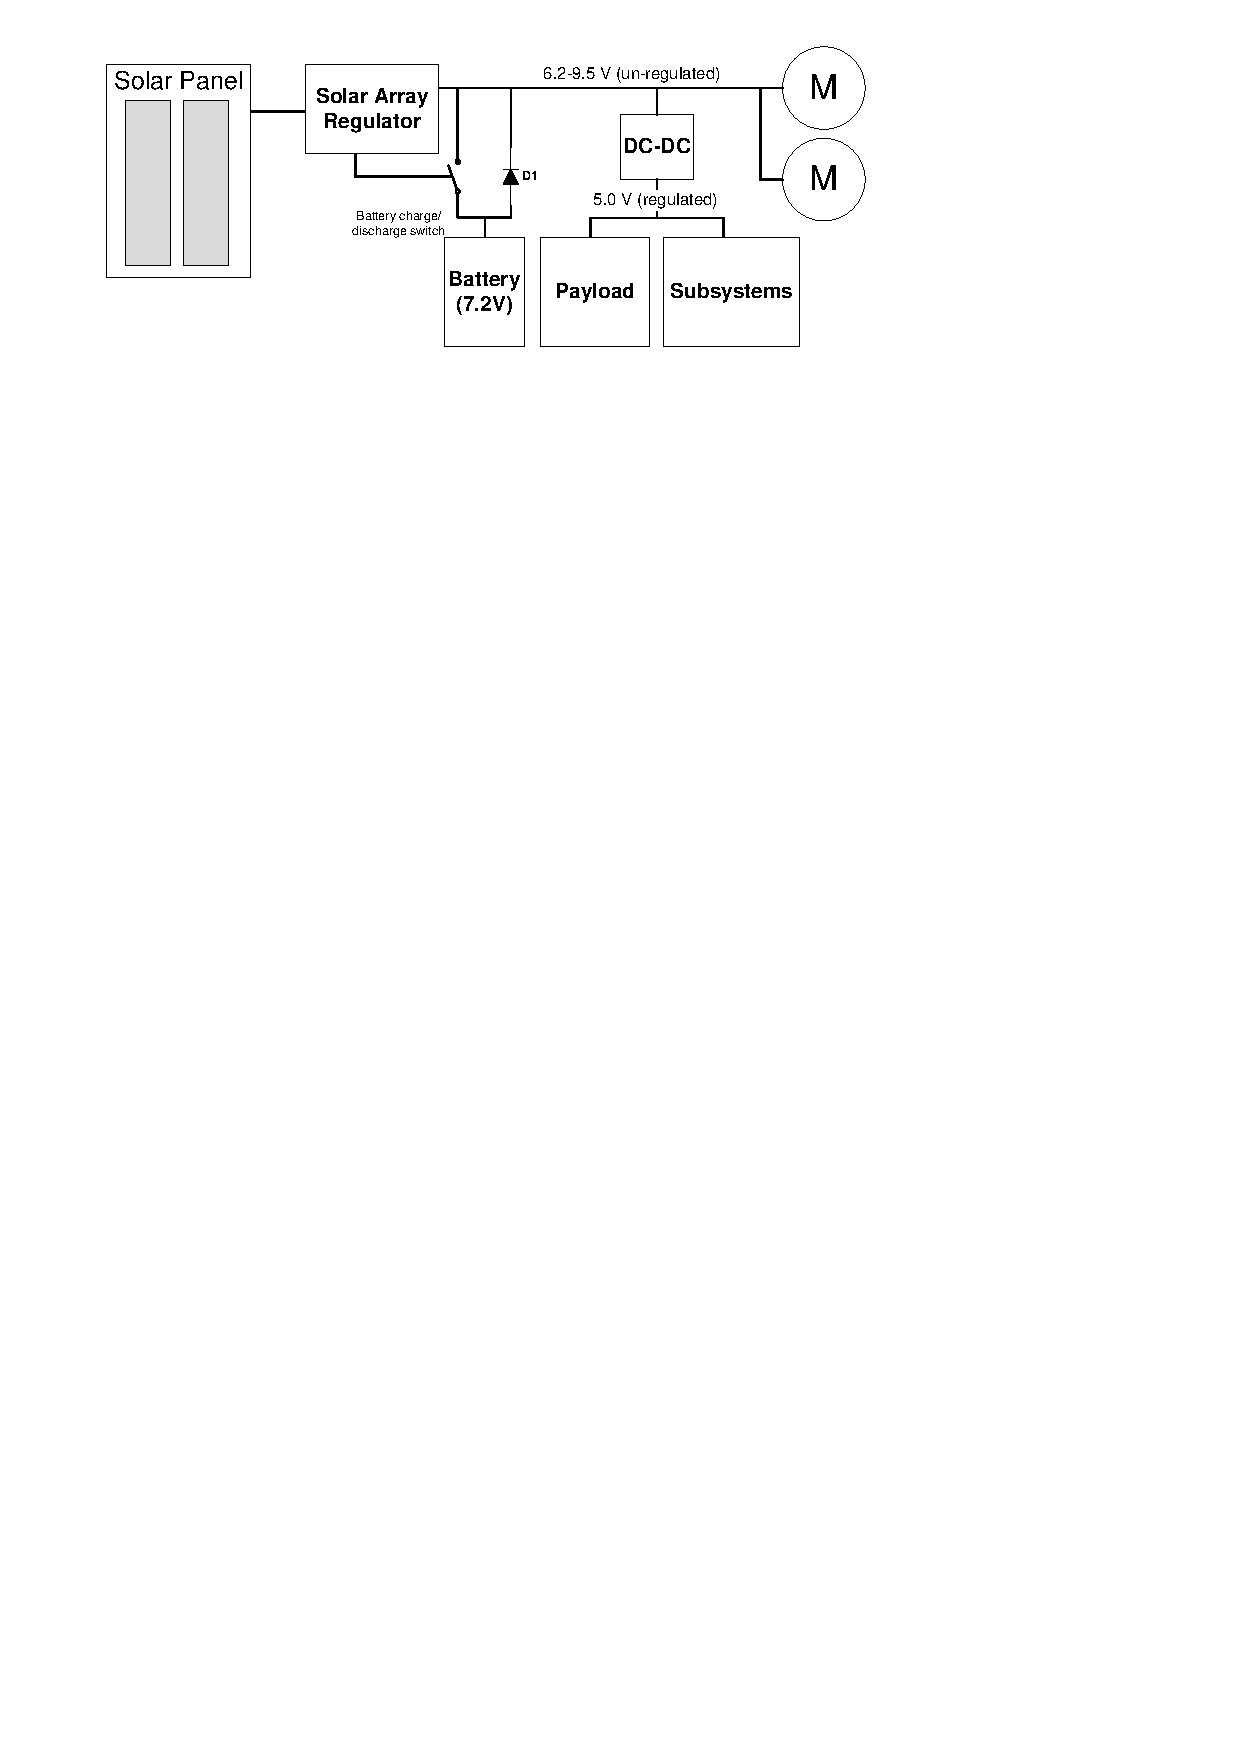
\includegraphics[width=\textwidth]{figures/fig_PDR_EPSdiagram}
\caption{\ac{EPS} simple blockdiagram}
\label{fig:EPS_diagram_simple}
\end{figure}
%
%
\subsection{Battery Design}
In \cite{PDR} it was decided that a Li-ion type battery was suitable for the \ac{EPS}. An \textit{Ansmann \ac{LiPo} Racing Pack 2S1P 30C} battery is selected with the specifications as listed in Table \ref{tab:proposed_battery}.
%
\begin{table}[H]
\centering
\caption{Specification of chosen battery}
\label{tab:proposed_battery}
\begin{tabular}{p{0.35\textwidth}p{0.15\textwidth}p{0.4\textwidth}}
\hline
\textbf{Description} & \textbf{Symbol} & \textbf{Value}\\
\hline 
Chemistry & - & Li-Polymer\\
Nominal voltage & $V_{bat}$ & $7.4\,V$\\
Capacity & $C_{bat}$ & $2.1\,Ah$ / $15.54\,Wh$\\
Weight & $W_{bat}$ & $122\,g$\\
Dimensions & - & $105\,mm\:\times\:35.2\,mm\:\times\:17\,mm$\\
Maximum fast charge current & $I_{charge,max}$ & $3\,A$\\
Maximum discharge current (continuous) & $I_{discharge,max}$ & $63\,A$\\
\hline
\end{tabular}
\end{table}
%
%
\subsubsection{Battery Charge Regulator}
\label{subsec:BCR}
%
The \ac{BCR} must control the charge rate of the battery such that the charge current limit is not exceeded and cut off the charge current when the battery is fully charged. Temperature monitoring is usually also required to inhibit charging if the battery temperature is outside its safety limits. 


An \textit{MCP73842} Li-ion battery charge regulator \ac{IC} is selected. It employs three different charge modes: low-charge for deeply discharged batteries, \ac{CC} charge and trickle charging as well as inputs for temperature monitoring. The battery maximum charge current was in Table \ref{tab:proposed_battery} given as $3\,A$. From the \textit{MCP73842} datasheet, the minimum current sense resistor value is calculated as
%
\begin{equation}
\begin{split}
R_{sense}=&\dfrac{V_{FCS}}{I_{REG}}\\
R_{sense}=&\dfrac{120\,mV}{3\,A}=40\,m\Omega
\end{split}
\end{equation}
%
A $50\,m \Omega$ current sense resistor is selected leading to a charge current of $2.4\,A$.
%
The worst-case thermal dissipation in the MOSFET happens when the battery is charged from its minimum charge state
%
\begin{equation}
P_{max,MOSFET}=(V_{in,max}-V_F-V_{bat,min})\cdot I_{charge}=(9.5\,V-0.3\,V-5.5\,V)\cdot 2.4\,A=8.88\,W
\end{equation}
%
where $V_{in,max}$ is the maximum mainbus voltage, $V_F$ the expected Schottky diode forward voltage drop and $V_{bat,min}$ is the preconditioning threshold voltage of the \ac{BCR} \ac{IC}.
An \textit{SUP75P03-07-E3} P-channel MOSFET is selected which is rated for a peak power dissipation of $187\,W$, well above the minimum requirement provided that suitable thermal design is applied, most likely also including a heat sink. 
\\[2mm]
Calculations on heat sink requirements still remain to be done.
%
\subsubsection*{Future Improvements}
As was calculated above, significant power may be lost in the \ac{BCR} MOSFET. This is due to the selected \ac{BCR} \ac{IC} which requires an input voltage of around $9.5\,V$ (including a Schottky diode forward voltage drop and some design margin). In future, the \ac{BCR} could be designed to allow operation with an input voltage only slightly above the battery voltage thus minimizing the charge losses and the thermal requirements of the MOSFET.
%
%
\subsubsection{Battery Temperature Monitoring}
%%
The selected \ac{LiPo} battery is rated, in charge-mode, for the temperature interval $0$ to $+45^{\circ}C$. For temperature measuring, a $4.7\,k \Omega$ \textit{NTCLE203E3472GB0} thermistor is selected which has a Beta Value, $B=3977\,K$. Since the battery temperature is measured using an external thermistor, thus the temperature response is likely to be somewhat slower, an extra $5^{\circ}C$ thermal design margin is added. The required resistance values of the \ac{BCR} temperature control resistors are determined from the \textit{MCP73842} datasheet as 
%
\begin{equation}
\begin{split}
R_{cold}&=R_{25}\,e^{B(\dfrac{1}{T}-\dfrac{1}{T_0})}=4.7\,k\Omega \,e^{3977\,K(\dfrac{1}{278	\,K}-\dfrac{1}{298\,K})}=12.28\,k\Omega\\
R_{hot}&=4.7\,k\Omega \, e^{3977\,K(\dfrac{1}{313	\,K}-\dfrac{1}{298\,K})}=2.48\,k\Omega\\
R_{T1}&=2\dfrac{R_{cold}R_{hot}}{R_{cold}-R_{hot}}=6.2\,k\Omega\\
R_{T2}&=2\dfrac{R_{cold}R_{hot}}{R_{cold}-3R_{hot}}=12.6\,k\Omega
\end{split}
\end{equation}
%
where $R_{25}$, $R_{cold}$ and $R_{hot}$ are the thermistor resistance values at room temperature, the low and high temperature limits respectively. $R_{T1}$ and $R_{T2}$ are the required \ac{BCR} temperature control resistors setting the required temperature interval.

If the sensed battery temperature falls outside the $+5$ to $+40^{\circ}\,C$ region, battery charging will be inhibited. The technical requirements from Table \ref{tab:technical_requirements} requires the \ac{EPS} to operate down to $-20^{\circ}\,C$. Hence some insulation and/or heating of the battery may be necessary or flight must be disallowed at outdoors temperatures much below $+5^{\circ}\,C$.
%
\subsubsection{Battery Under-Voltage Lock-Out}
To prevent over-discharge of the battery, a battery \ac{UVLO} circuit is added as shown in Figure \ref{fig:EPS_diagram_detailed}. An \textit{TL431} precision shunt regulator \ac{IC} is selected. The lock-out voltage is given as
%
\begin{equation}
V_{UVLO}=V_{ref}(1+\dfrac{R_1}{R_2})=2.5\,V(1+\dfrac{29\,k \Omega}{20\,k \Omega})=6.125\,V
\end{equation}
%
where $V_{ref}$ is the \textit{TL431} build-in voltage reference. If the battery voltage drops below this value, the gate voltage to the P-type MOSFET is pulled high thus opening the switch. The $1\,M \Omega$ resistor adds about $200\,mV$ hysteresis. 

The \ac{UVLO} circuit only cuts out the motor power line. Thus payloads remain supplied and the battery is still slowly drained. This design has been chosen to allow  telemetry and telecommand capability during a heavy battery discharge event. In this case, it is expected that all payloads and on-board computers enter a low power consumption mode, to extend the remaining battery supply time. If the battery voltage drops below $5.62\,V$, the $5\,V$ payload power supply shuts down and all telemetry and telecommand capabilities will be lost.
%
\subsection{Solar Array Design}
\label{sec:SA}
The main driver for selecting the solar cell is to choose a part which is very light-weight and easy to mount on the \ac{SPA}. A  \textit{PowerFilm RC7.2-75(PSA)} solar cell is selected as shown in Figure \ref{fig:solar_cell}. This is a very light-weight flexible solar cell with a \ac{PSA} backside for mounting. Table \ref{tab:solar_cell_spec} lists the solar cell specifications.
%
\begin{table}[H]
\centering
\caption{Specifications of chosen solar cell}
\label{tab:solar_cell_spec}
\begin{minipage}{\textwidth}
\begin{tabular}{p{0.35\textwidth}p{0.15\textwidth}p{0.4\textwidth}}
\hline
\textbf{Description} & \textbf{Symbol} & \textbf{Value}\\
\hline
Nominal output current & $I_{cell}$ & $100\,mA$\\
Nominal output voltage & $V_{cell}$ & $7.2V$\\
Nominal output power & $P_{cell}$ & $0.72\,W$\\
Dimensions & - & $270\,mm\:\times\:90\,mm\:\times\:0.2\,mm$\\
Weight & $W_{cell}$ & $7.6\,g$\\
No. of required cells & $N_{cells}$ & $100$\footnote{\cite{avnetexpress} offers good discount for +100 units order}\\
Total solar array area & $A_{array}$ & $2.43\,m^2$ (assuming $100\,\%$ fill factor)\\
\hline
\end{tabular}\par
\vspace{-0.75\skip\footins}
\renewcommand{\footnoterule}{}
\end{minipage}
\end{table}
%
The solar array is an array of 50 parallel connected strings of two series solar cells as shown in Figure \ref{fig:solar_cell}. The nominal output voltage and current are given as
%
\begin{equation}
\begin{split}
V_{array}&=2\cdot V_{cell}=14.4\,V\\
I_{array}&=50\cdot I_{cell}=5\,A
\end{split}
\end{equation}
%
\begin{figure}[H]
\centering
\begin{minipage}[t]{0.4\linewidth}
\centering
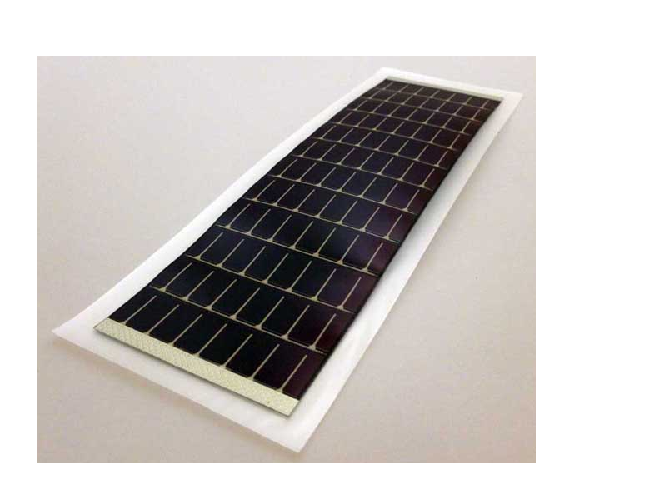
\includegraphics[width=1\textwidth]{figures/SolarCell_RC7-2_Powerfilm}
\end{minipage}
\hspace{5mm}
\begin{minipage}[t]{0.55\linewidth}
\centering
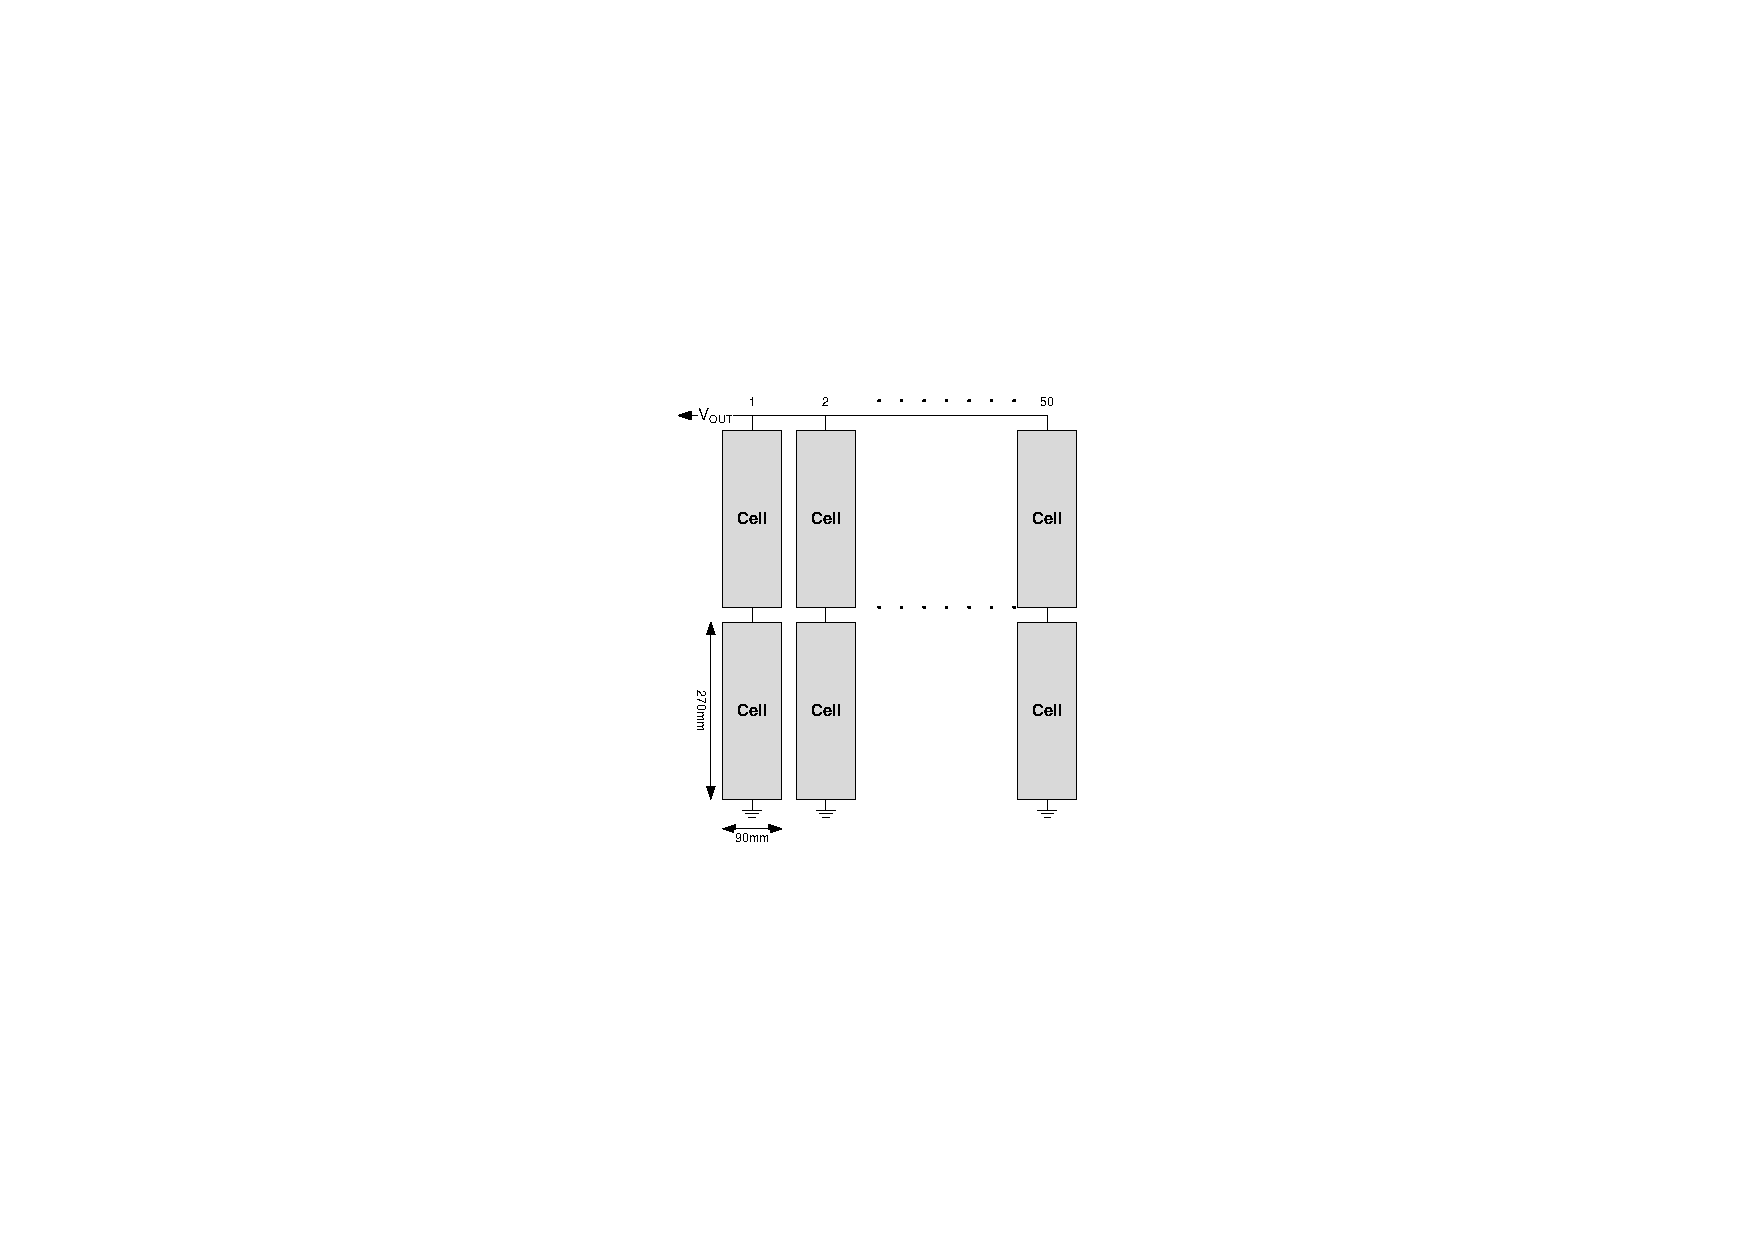
\includegraphics[width=\textwidth]{figures/fig_CDR_Solar_Array}
\end{minipage}
\caption{PowerFilm solar cell(left), solar array configuration(right)}
\label{fig:solar_cell}
\end{figure}
%
Since only two cells are in series, it is estimated that bypass diodes are not very beneficial for mitigating shading issues, as was discussed in Section \ref{subsec:environmental_requirements}, and hence are not included in the design.
%
\subsection{Solar Array Regulator}
The \ac{SAR} must control the optimal the solar array operating voltage as well as limit the output mainbus voltage. A simple step-down buck converter topology is preferred for a number of reasons:
%
\begin{itemize}
\item simple circuit analysis and low components count
\item no inherent \ac{RHPZ} in contrary to the standard boost topology
\item step-down topology calls for a high input voltage which leads to low input current thus minimizing ohmic losses and the relative forward voltage drop loss from the reverse protection diode
\end{itemize}
%
\subsubsection{Buck Converter Circuit Design}
The ideal transfer function for the buck converter shown in Figure \ref{fig:EPS_diagram_detailed} is given as
%
\begin{equation}
V_{out}=D\,V_{in}
\end{equation}
%
where $D$ is the duty cycle of the MOSFET switch, $V_{in}$ the solar array voltage and $V_{out}$ the mainbus voltage. The duty cycle is controlled by a \ac{PWM} controller which provides input to a high-side MOSFET driver. A \ac{MEA} measures the mainbus output voltage to generate a control signal for the PWM controller. An \textit{LM3477} chip is selected which combines \ac{PWM} controller, \ac{MEA} and gate driver in one \ac{IC}.

The \ac{CM} control scheme is adopted due to its excellent dynamic abilities\cite[sec. 12-3-6]{Fundamentals} and simplified feedback regulator design. A low resistance $10\,m \Omega$ precision sense resistor measures the inductor current slope. The \textit{LM3477} has build-in slope compensation to avoid current mode instabilities\cite[sec. 12-1]{Fundamentals}.

The converter switching frequency, $f_{switch}$, is chosen relatively high to $500\,kHz$. The increased switching losses are expected to by out-weighted by the fact that the low operating voltage limits switching losses and high frequency allows the inductor and filter components to be made smaller thus limiting system mass and the resistive losses in the inductor copper wires which are expected to dominate converter losses due to the relatively high currents.


The inductor current ripple, $\Delta I_L$, can be calculated as 
%
\begin{equation}
\Delta I_L=\dfrac{V_{in}-V_{out}}{L\,f_{switch}}D
\end{equation}
%
where $L$ is the inductance and $f_{switch}$ the converter switching frequency. The inductor current ripple is usually limited to about $10\,\%$ of the maximum output current which was given in Table \ref{tab:technical_requirements} as $10.8\,A$. Thus the minimum required inductance is calculated to
%
\begin{equation}
L=\dfrac{V_{in}-V_{out}}{\Delta I_L\,f_{switch}}D=\dfrac{14.4\,V-7.4\,V}{1.08\,A\cdot 500\,kHz}\cdot 0.514=6.7\,uH
\end{equation}
%
A $10\,uH$ inductor is chosen giving a current ripple of about $0.72\,A$. If the load current drops below $0.36\,A$, which is unlikely to happen in most operating modes, the converter will enter \ac{DCM}.

For the converter output capacitor, a component is chosen which has very low \ac{ESR} and high capacitance to limit the output voltage ripples.
%
\subsubsection*{Current Sense Amplifier}
With an inductor current ripple of $0.72\,A$ the current sense voltage slope is only 
%
\begin{equation}
v_{sense}=\Delta I_L\cdot R_{sense}=0.72\,A\cdot 10\,m\Omega = 7.2\,mV
\end{equation}
%
It is recommended that the slope compensation is equal to or the double of the sense slope\cite[sec. 12-1]{Fundamentals}, however the minimum compensation slope is limited to $103\,mV$ by the \textit{LM3477} chip. Thus the sensed slope signal must be amplified with a gain of around 20 being suitable. This also has the advantage of eliminating some of the typical noise susceptibility in the current sense signal. The current sense circuit in Figure \ref{fig:EPS_diagram_detailed} consists of two differential OpAmps which amplifies the current sense slope. Resistive voltage dividers are placed on the OpAmp inputs to scale down the input voltage signals to always be below the $5\,V$ OpAmp supply voltage.
%
\subsubsection*{Input Filter}
An input filter is placed in front of the buck converter, mainly to draw a continuous current from the solar array. It also reduces the converter \ac{EMC} issues. 
One challenge with the input filter is that it effects the dynamic properties of the converter and if not properly designed, it can degrade the control feedback loop performance. A damping network in the filter is also necessary to avoid instabilities\cite[sec. 10-3]{Fundamentals}.

A usable filter has been designed based on PSpice simulations. However thorough analysis still remains to be done to optimize the filter design.
%
%
\subsubsection{Maximum Power Point Tracker Unit}
\label{sec:MPPTU}
In \cite{PDR} it was decided to use a \ac{MPPTU} with the \ac{SAR} to increase solar array efficiency during changing environment conditions.
%
The \ac{SAR} with \ac{MPPT} can operate in three different operation regions:
%
\begin{itemize}
\item Battery discharge - when the solar array input power is insufficient to cover the load power demand, the battery is slowly discharged in order to maintain the output voltage. The \ac{MPPTU} controls the input solar array voltage.
\item Battery charge - when the solar array input is greater than the load power, excessive power is used to recharge the battery. The \ac{MPPTU} controls the input solar array voltage.
\item Input power limitation - when the battery is fully charged, the regulator will operate the solar array at a non-optimal voltage, thus limiting the input power to keep the output voltage at a maximum limit. The extra potential input power is dissipated as heat externally on the solar arrays.
\end{itemize}
%
It is preferred to implement an analog \ac{MPPTU} mainly since this makes the circuit independent on a control signal from a more complicated external \ac{MCU} or \ac{DSP} thus allowing a flexible plug'n-play system to be implemented. One challenge with an analog \ac{MPPTU} is the typical need for expensive analog multipliers\cite{Liang}. Since the required multiplier only needs to be a 1st quadrant type (only two positive inputs), it is believed that a low-cost multiplier can be build using standard discrete components\cite{Multiplier}.
%
\\[2mm]
The \ac{MPPTU} design still remains to be completed.
%
%
\subsubsection{Mode Transitions}
%
As was discussed in Section \ref{sec:MPPTU}, the \ac{SAR} can operate in three different main modes. The transition between the modes is controlled by the mainbus output voltage as shown in Figure \ref{fig:SAR_ModeTransition}. If the \ac{SAR} input power is lower than the load power, the battery will discharge and the mainbus voltage will follow the battery voltage. Once the input power is larger than the load power, the mainbus capacitor will quickly be charged to a voltage higher than the battery voltage. Once the mainbus capacitor voltage crosses the $9.2\,V$ charge threshold, the \ac{BCR} starts to charge the battery. If the input power is still higher than the combined battery charge power and load power, the mainbus capacitor voltage continues to rise until reaching $9.5\,V$ where the \ac{SAR} enters the input power limitation mode. The battery may still be charging in this mode. Since the battery is charged with constant current, the input power may be lower than the combined charge and load power but higher than the load power alone. Hence an oscillatory state between battery charge and discharge mode may rise whose frequency depends on the mainbus capacitance which should therefore be large. 

The $9.20\,V$ battery charge threshold voltage is calculated from
%
\begin{equation}
V_{charge,threshold}=V_{UVLO,BCR}+V_F=8.90\,V+0.3\,V= 9.20\,V
\end{equation}
%
where $V_{UVLO,BCR}$ is the worst-case \ac{UVLO} threshold voltage of the \ac{BCR} \ac{IC} and $V_F$ is the reverse protection diode forward voltage drop.
%
%
\begin{figure}[H]
\centering
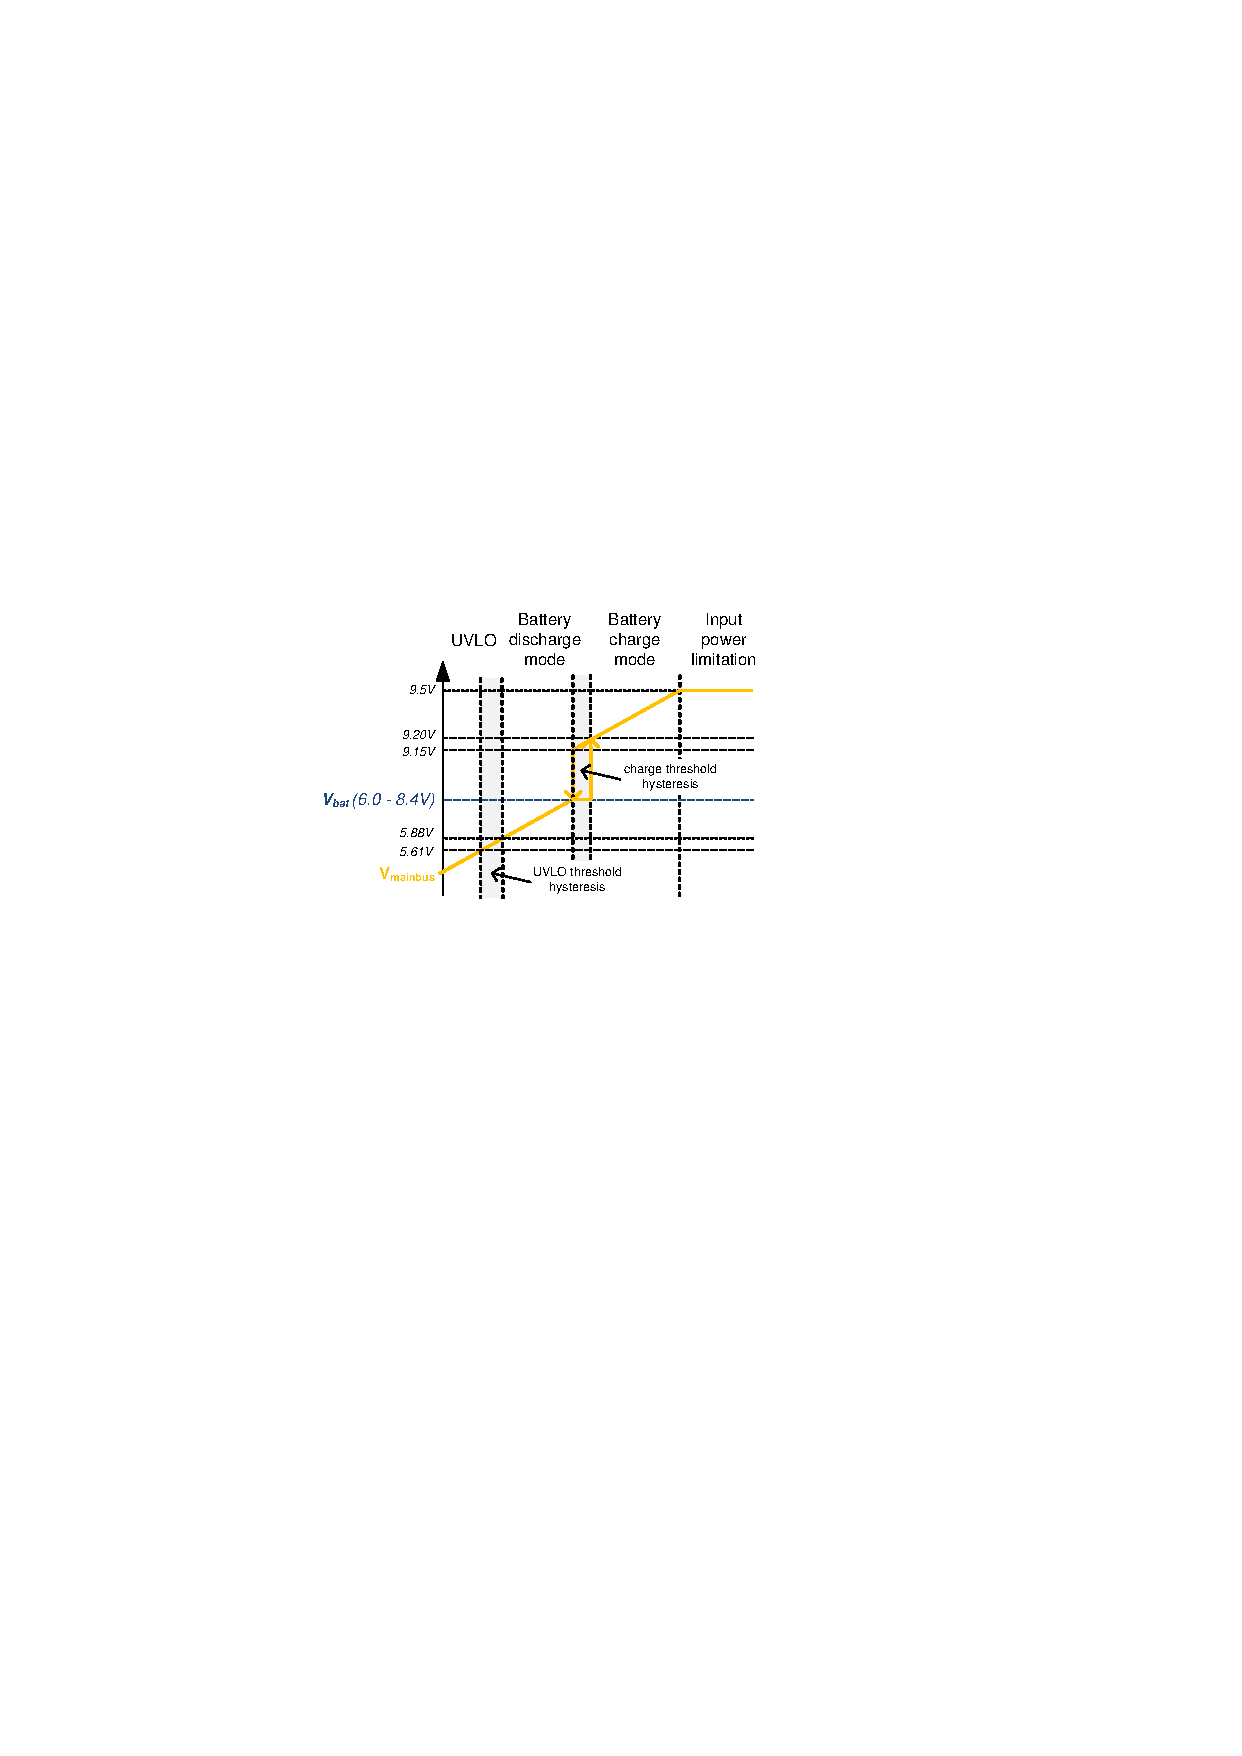
\includegraphics[width=0.8\textwidth]{figures/fig_CDR_SAR_ModeTransition}
\caption{Different \ac{SAR} operation modes as function of mainbus voltage}
\label{fig:SAR_ModeTransition}
\end{figure}%
%
%
\subsection{5V Regulator}
To provide a regulated $5\,V$ supply for the on-board computer and payloads, a \textit{MIC29300-5} \ac{LDO} regulator is selected. A $2\,A$ resettable \ac{PTC} fuse is added to protect the loads from excessive currents and to protect the battery in case of a payload short-circuit failure.
%
\subsection{Complete Electrical Power System Diagram}
%
The complete \ac{EPS} diagram is shown in Figure \ref{fig:EPS_diagram_detailed}. Two $17\,A$ fuses are added in front of the motors, to protect the battery from a motor short-circuit failure.
%
\begin{sidewaysfigure}
\centering
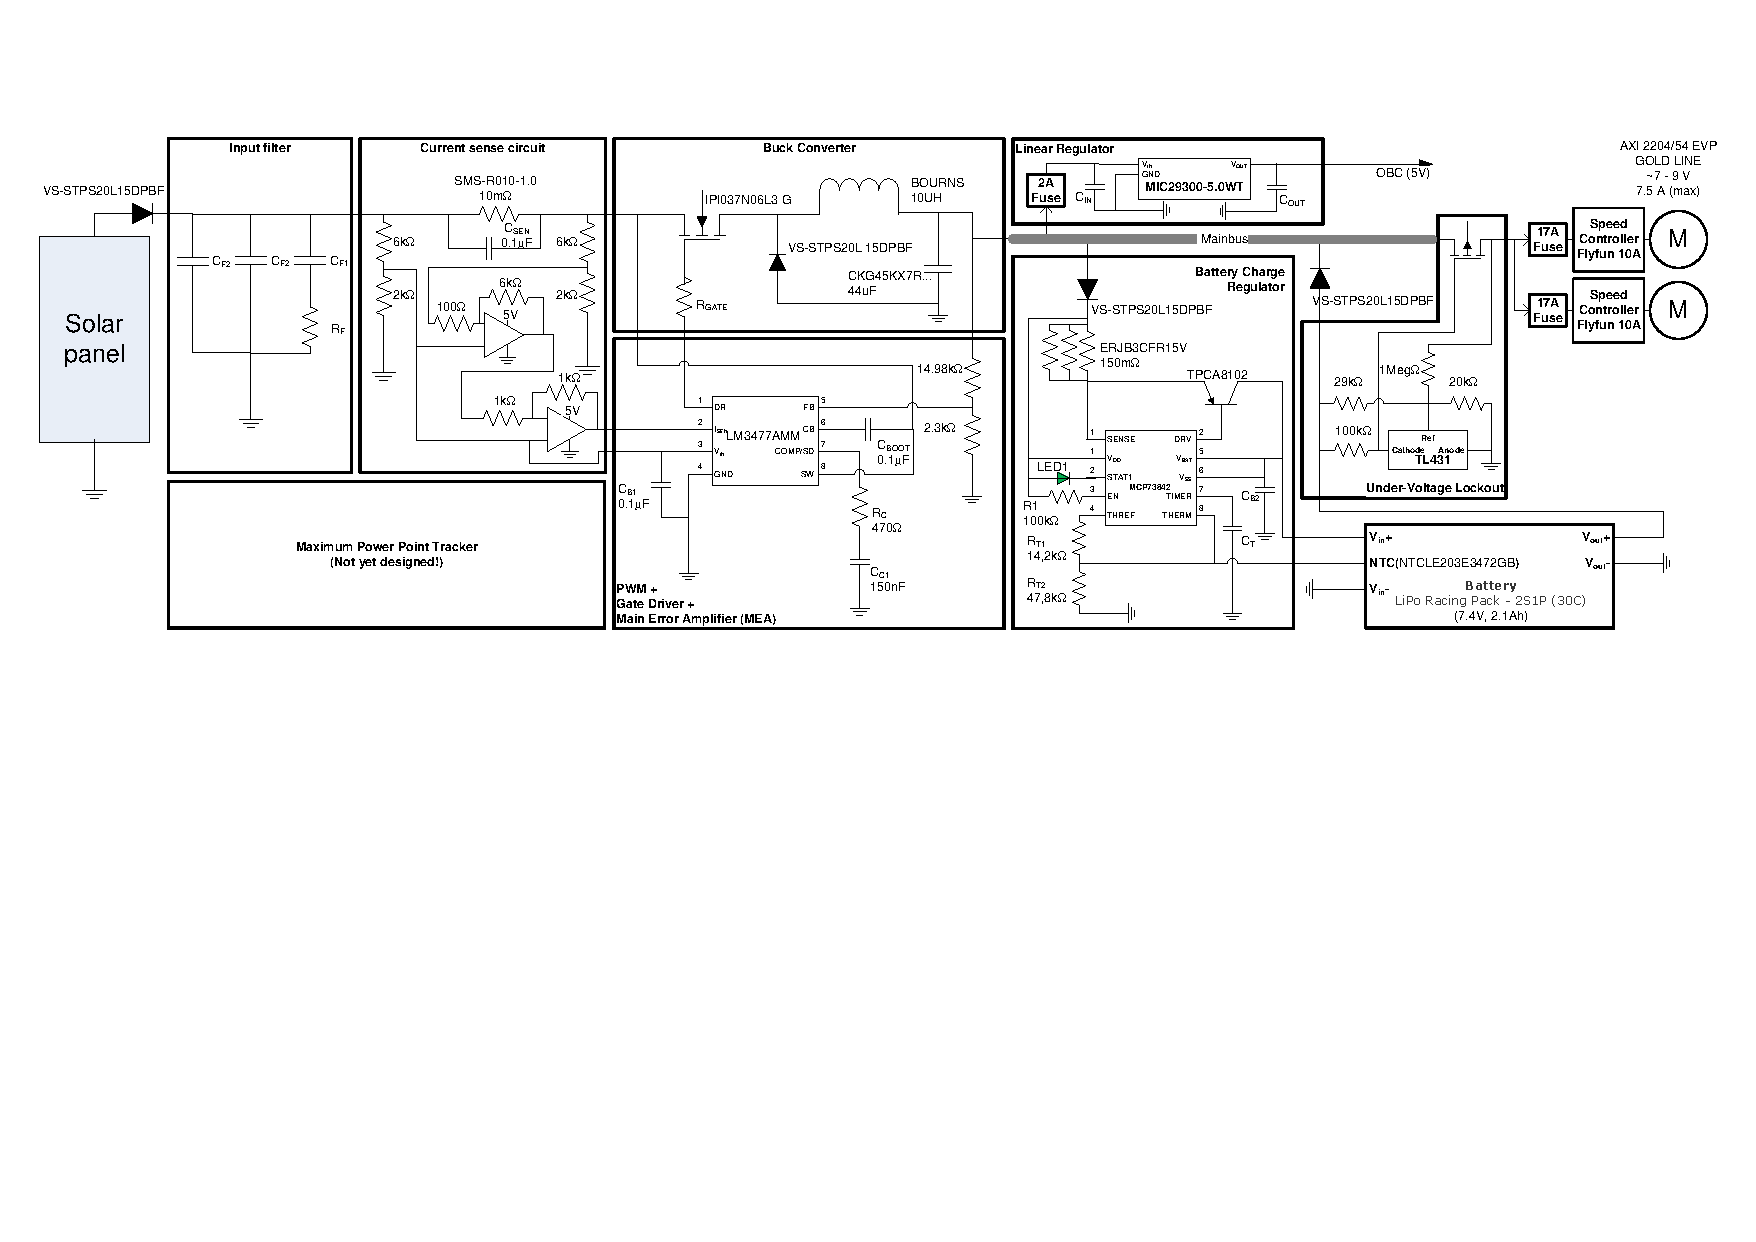
\includegraphics[scale=0.8]{figures/fig_CDR_EPSdiagram_detailed}
\caption{\ac{EPS} detailed block diagram}
\label{fig:EPS_diagram_detailed}
\end{sidewaysfigure}

%
\subsection{External Interfaces}
%
The interfaces of the \ac{EPS} external are listed in table \ref{tab:external_interfaces}.
%
\begin{table}[H]
\centering
\caption{External interfaces}
\label{tab:external_interfaces}
\begin{tabular}{m{0.3\textwidth}m{0.15\textwidth}m{0.45\textwidth}}
\hline
\textbf{External interface} & \textbf{Type} & \textbf{Implementation}\\
\hline
Solar cells mounting & Mechanical & \ac{TBD} (possibly using \ac{PSA})\\[2mm]
Power electronics mounting & Mechanical & Mounted on a \ac{PCB} which sits in the cargo bay, attached with screws\\[2mm]
Battery mounting & Mechanical & Mounted in cargo bay with strips or Velcro. Thermal insulation with styrofoam or similar material should be added to protect against cold temperatures.\\[2mm]
\ac{EPS} telemetry & Electrical & Analog signals to Microcontroller. Electrical connector interface still remains \ac{TBD}\\[2mm]
\ac{EPS} telecommands & Electrical & \ac{TBD}\\[2mm]
Output voltages & Electrical & $6.0-9.5\,V$ (unregulated) and $5.0\,V$(regulated)\\[2mm]
\hline
\end{tabular}
\end{table}
%
%
\subsection{Telemetry and Telecommands}
The suggested \ac{EPS} telemetries are listed in Table \ref{tab:Telemetry} and the suggest telecommands in Table \ref{tab:Telecommands}. Not all telemetries or the telecommands are part of the initial \ac{EPS} design and will only be implemented if time and ressources allow it.

The exact electrical configuration and interface connectors still remains to be designed.
%
\begin{table}[H]
\centering
\caption{\ac{EPS} telemetry}
\label{tab:Telemetry}
%\begin{minipage}{\textwidth}
\begin{tabular}{|p{0.29\textwidth}p{0.13\textwidth}p{0.13\textwidth}p{0.35\textwidth}|}
\hline
\textbf{Telemetry} & \textbf{Data rate} & \textbf{Data size} & \textbf{Data range}\\
\hline
Battery voltage & Every 5 sec & 2 bytes & \ac{TBD}\\
\hline
Battery temperature & Every 5 sec & 2 bytes & \ac{TBD}\\
\hline
BCR status & Every 5 sec & 1 byte & high($5\,V$), low($0\,V$) and $1\,Hz\;50\%$ duty cycle ripple\footnote{for explanation of the different status indications, look in the \ac{BCR} \ac{IC} datasheet}\\
\hline
\ac{UVLO} status & Every 5 sec & 1 byte &  $0\,V$(nominal operation), $5\,V$(under-voltage lock-out)\\
\hline
Mainbus voltage & Every 5 sec & 2 bytes & \ac{TBD}\\
\hline
Solar array temperature & Every 5 sec & 2 bytes & \ac{TBD}\\
\hline
Solar array voltage & Every 1 sec & 2 bytes & \ac{TBD}\\
\hline
\end{tabular}
\end{table}
%
\begin{table}[H]
\centering
\caption{\ac{EPS} telecommands}
\label{tab:Telecommands}
%\begin{minipage}{\textwidth}
\begin{tabular}{|p{0.25\textwidth}p{0.25\textwidth}p{0.45\textwidth}|}
\hline
\textbf{Telecommand} & \textbf{Command format} & \textbf{Description}\\
\hline
Battery charge inhibit & \ac{TBD} & Battery charging can be remotely terminated in case of battery anomalies\\
\hline
Solar array voltage set & \ac{TBD} & When \ac{MPPT} is running, the solar array operating voltage can manually be set to mitigate any malfunction in the \ac{MPPT} algorithm\\
\hline
\end{tabular}
\end{table}